%%%%%%%%%%%%%%%%%%%%%%%%%%%%%%%%%%%%%%%%%%%%%%%%%%%%%%%%%%%%%%%%%%%%%%%%%%%%%
%%%
%%% File: thesis.tex, version 1.9, May 2016
%%%
%%% =============================================
%%% This file contains a template that can be used with the package
%%% cs.sty and LaTeX2e to produce a thesis that meets the requirements
%%% of the Computer Science Department from the Technical University of Cluj-Napoca
%%%%%%%%%%%%%%%%%%%%%%%%%%%%%%%%%%%%%%%%%%%%%%%%%%%%%%%%%%%%%%%%%%%%%%%%%%%%%

%!TEX TS-program = xelatex
%!TEX encoding = UTF-8 Unicode
\documentclass[12pt,a4paper,twoside]{report}    

\usepackage{fontspec,xltxtra,xunicode}
\defaultfontfeatures{Mapping=tex-text}
\setmainfont[Mapping=tex-text]{Times New Roman}
     
\usepackage{cs}              
%\usepackage{times}
\usepackage{graphicx}
\usepackage{latexsym}
\usepackage{amsmath,amsbsy}
\usepackage{amssymb}
\usepackage[matrix,arrow]{xy}
%\usepackage[T1]{fontenc}
%\usepackage{ae,aecompl}
\usepackage{romanian} %definitii pentru diacritice; 
\usepackage{amstext}
\usepackage{graphics}
%\usepackage[T1]{fontenc}
%\usepackage{ae,aecompl}
\usepackage{algorithm}
\usepackage{color}
%\usepackage{color}


% \mastersthesis
\diplomathesis
% \leftchapter
\centerchapter
% \rightchapter
\singlespace
% \oneandhalfspace
% \doublespace

\renewcommand{\thesisauthor}{Bogdan Daniel ARDELEAN}    %% Your name.
\renewcommand{\thesismonth}{Iunie}     %% Your month of graduation.
\renewcommand{\thesisyear}{2017}      %% Your year of graduation.
\renewcommand{\thesistitle}{FPWAM - O implementare a mașinii abstracte Warren pe FPGA} % Title
\renewcommand{\thesissupervisor}{Dr. Ing. Zoltan Francisc BARUCH}
\newcommand{\department}{FACULTATEA DE AUTOMATIC'A 'SI CALCULATOARE\\
DEPARTAMENTUL CALCULATOARE}
\newcommand{\thesis}{LUCRARE DE LICEN'T'A}
\newcommand{\uline}[1]{\rule[0pt]{#1}{0.4pt}}
%\renewcommand{\thesisdedication}{P'arin'tilor mei}
\newcommand{\utcnlogo}{
\includegraphics[width=15cm]{img/utcn.jpg}}

\begin{document}
%\frontmatter
%\pagestyle{headings}

\newenvironment{definition}[1][Defini'tie.]{\begin{trivlist}
\item[\hskip \labelsep {\bfseries #1}]}{\end{trivlist}}



%\thesistitle                    %% Generate the title page.
%\authordeclarationpage                %% Generate the declaration page.

\pagenumbering{arabic}
\setcounter{page}{4}



\begin{center}
%\includegraphics[width=15cm]{img/tucn.jpg}  
\utcnlogo

{\bf \department}

\vspace{4cm}

{\bf \thesistitle} %LICENSE THESIS TITLE}

\vspace{1.5cm}

\thesis

\vspace{6cm}

Absolvent: {\bf \thesisauthor} 

Conduc'ator 'stiin'tific: {\bf \thesissupervisor}

\vspace{3cm}
{\bf \thesisyear}
\end{center}

\thispagestyle{empty}
\newpage

\begin{center}
\utcnlogo

{\bf \department}
\end{center}
\vspace{0.5cm}

%\begin{small}
\begin{tabular}{p{7cm}p{8cm}}
 %\hspace{-1cm}& VIZAT,\\
 \hspace{-1cm}DECAN, & DIRECTOR DEPARTAMENT,\\
\hspace{-1cm}{\bf Prof. dr. ing. Liviu MICLEA} & {\bf Prof. dr. ing. Rodica POTOLEA}\\  
\end{tabular}
 
\vspace{2cm}

\begin{center}
Absolvent: {\bf \thesisauthor}

\vspace{1cm}

{\bf \thesistitle}
\end{center}

\vspace{1cm}

\begin{enumerate}
 \item {\bf Enun'tul temei:} {\it Scurt'a descriere a temei lucr'arii de licen't'a 'si datele ini'tiale}
\item {\bf Con'tinutul lucr'arii:} {\it (enumerarea p'ar'tilor componente) Exemplu: Pagina de prezentare, aprecierile coordonatorului de lucrare, titlul capitolului 1, titlul capitolului 2, titlul capitolului n, bibliografie, anexe.}
\item {\bf Locul document'arii:} {\it Exemplu}: Universitatea Tehnic'a din Cluj-Napoca, Departamentul Calculatoare
\item {\bf Consultan'ti:}
\item {\bf Data emiterii temei:} 1 Noiembrie 2015
\item {\bf Date pred'arii:} 17 Februarie 2017 {\it (se va completa data pred'arii)}
  \end{enumerate}
\vspace{1.2cm}

\hspace{6cm} Absolvent: \uline{6cm} 

\vspace{0.5cm}
\hspace{6cm} Coordonator 'stiin'tific: \uline{5cm} 
%\end{small}

\thispagestyle{empty}


\newpage
$ $
%\begin{center}
%\utcnlogo

%{\bf \department}
%\end{center}

\thispagestyle{empty}
\newpage

\begin{center}
\utcnlogo

{\bf \department}
\end{center}

\vspace{0.5cm}

\begin{center}
{\bf
Declara'tie pe proprie r'aspundere privind\\ 
autenticitatea lucr'arii de licen't'a}
\end{center}
\vspace{1cm}



Subsemnatul(a) \\
\uline{14.8cm}, 
legitimat('a) cu \uline{4cm} seria \uline{3cm} nr. \uline{4cm}\\
CNP \uline{9cm}, autorul lucr'arii \uline{2.8cm}\\
\uline{16cm}\\
\uline{16cm}\\
elaborat'a 'in vederea sus'tinerii examenului de finalizare a studiilor de licen't'a la Facultatea de Automatic'a 'si Calculatoare, Specializarea \uline{7cm} din cadrul Universit'a'tii Tehnice din Cluj-Napoca, sesiunea \uline{4cm} a anului universitar \uline{3cm}, declar pe proprie r'aspundere, c'a aceast'a lucrare este rezultatul propriei activit'a'ti intelectuale, pe baza cercet'arilor mele 'si pe baza informa'tiilor ob'tinute din surse care au fost citate, 'in textul lucr'arii 'si 'in bibliografie.

Declar, c'a aceast'a lucrare nu con'tine por'tiuni plagiate, iar sursele bibliografice au fost folosite cu respectarea legisla'tiei rom\ia ne 'si a conven'tiilor interna'tionale privind drepturile de autor.

Declar, de asemenea, c'a aceast'a lucrare nu a mai fost prezentat'a 'in fa'ta unei alte comisii de examen de licen't'a.

'In cazul constat'arii ulterioare a unor declara'tii false, voi suporta sanc'tiunile administrative, respectiv, \emph{anularea examenului de licen't'a}.

\vspace{1.5cm}

Data \hspace{8cm} Nume, Prenume

\vspace{0.5cm}

\uline{3cm} \hspace{5cm} \uline{5cm}

\vspace{1cm}
\hspace{9.4cm}Semn'atura

\thispagestyle{empty}

\newpage


%\listoftables
%\listoffigures

%\clearpage 
%\newpage

%\begin{comment}
\include{guideline} 
%\end{comment}

\newpage

\tableofcontents
\newpage



\chapter{Introducere - Contextul proiectului}
\label{chap:intro}
\pagestyle{headings}

%\begin{itemize}
%\item Contextul
%\item Conturarea domeniului exact al temei
%\item Reprezint'a cca. 5\% din lucrare
%\end{itemize}

\section{Contextul proiectului}
Încă din secolul XVII, cu mult înaintea calculatoarelor electronice, exista termenul \textit{calculator}. Până la jumătatea secolului XX, denotația lui era cu totul alta față de cea pe care o știm noi astăzi. Sensul acestui cuvânt referindu-se în principal la o meserie. Rolul asociat unei persoane care practica meseria de calculator, era de a efectua calcule matematice complexe în funcție de necesitățile clientului. Odată cu trecerea timpului, știința a avut întâmpinat provocări la care persoanele calculator nu mai puteau ține pasul. Această lipsă a puterii de calcul și inventarea tranzistorului au concentrat mediul industrial și academic în dezvoltarea sistemelor pe care astăzi le folosim zilnic.
\subsection{FPGA}
În momentul de față, majoritatea dispozitivelor de calcul existente au la bază un procesor cu scop general care execută un program croit după necesitățile utilizatorului. În ciuda imbunătățirilor constante și a flexibilității în dezvoltarea programelor acestor procesoare, arhitectura lor fixă nu se mulează întotdeauna suficient de mult pe problema pe care încearcă să o rezolve, rezultatul fiind nesatisfăcător din punctul de vedere a timpul de execuție și a amprentei energetice.\\
La jumătatea anilor 1980 a apărut primul circuit integrat comercial de tipul FPGA(Field-Programmable Gate Array)-referință. După cum le sugerează și numele, ele sunt niște circuite integrate care pot fi configurate de câte ori este nevoie de către utilizator. Avantajul acestor circuite este în principal natura lor paralelă și consumul redus de energie electrică. Datorită avansărilor tehnologice și prețului din ce în ce mai redus, ele au crescut în popularitate și au ajuns să fie folosite în multe domenii precum: \textit{Calcul de înaltă performanță, Auto, Audio, Medical, etc}. - referință
\subsection{Prolog}
Prolog a fost inventat la începutul anilor 1970 de către Alain Colmerauer și colegii lui de la Universitatea din Marseille-ref. El este printre primele limbaje de uz general care au ca paradigmă de baza programarea logică. Prima implementare a acestui limbaj a fost sub forma unui interpretor scris în FORTRAN chiar de către grupul din care Colmerauer făcea parte. Chiar și sub această formă rudimentară realizările au fost mari deoarece s-a demonstrat viabilitatea unui limbaj de programare logic. După aproximativ un deceniu, David H. D. Warren a rafinat și abstractizat principiile de implementare a limbajului sub forma unei mașini abstracte care este cunoscută astăzi sub numele de WAM. Majoritatea implementărilor de success ale limbajului Prolog folosesc ca referință de bază mașina abstractă mai sus amintită datorită simplității, eficienței și robusteții care au trecut testul timpului. Datorită popularității WAM, au fost scrise multe lucrări științifice care au adus îmbunătățiri arhitecturale a mașinii inițiale cât și multe extinderi. Una dintre cele mai sensibile subiecte este paralelizarea eficientă a acestei arhitecturi în speranța de a obține rezultate practice mai bune. \\
Prolog este de obicei asociat cu domeniul inteligenței artificiale și a lingvisticii computaționale. Cele mai des întâlnite aplicații ale limbajului fac parte din sfera mediului academic—e.g, sisteme expert, demonstrarea automată a teoremelor, NLP, planificare automată, etc.
\subsection{Nu m-am decis}
În contextul actual, atât domeniul circuitelor reconfigurabile, cât și domeniul inteligenței artificiale se dezvoltă cu un ritm accelerat, fiind folosite tot mai des în produse comerciale—e.g., aproape toate produsele Google folosesc elemente de inteligență artificială (Translate, Photos, etc.)-ref, Microsoft exploatează circuitele reconfigurabile pentru a accelera motorul de căutre BING-ref. În principiu orice aplicație care are la bază inteligența artificială are nevoie de un mediu de antrenare sau executare de înaltă performanță pe care procesoarele obișnuite nu îl pot oferi. Încercarea mea urmărește să utilizeze natura paralelă și performanța crescută a circuitelor FPGA, pentru a soluționa problema puterii de calcul în contextul aplicațiilor bazate pe limbajul Prolog.

%Se las'a un r\ia nd liber 'intre tabel 'si paragraful anterior, respectiv posterior (table~\ref{table:nonlin}).
%
%\begin{table}[ht]
%\caption{Rezultate}
%\centering                          % tabel centrat 
%\begin{tabular}{|c|c|c|c|}          % 4 coloane centrate 
%\hline\hline                        % linie orizontala dubla
%Case & Method\#1 & Method\#2 & Method\#3 \\ [0.5ex]   % inserare tabel
%%heading
%\hline                              % linie orizontal simpla
%1 & 50 & 837 & 970 \\               % corpul tabelului 
%2 & 47 & 877 & 230 \\
%3 & 31 & 25 & 415 \\[1ex]           % [1ex] adds vertical space
%\hline                              
%\end{tabular}
%  % titlul tabelului
%\label{table:nonlin}                % \label{table:nonlin} introduce eticheta folosita pentru referirea tabelului in text; referirea in text se va face cu \ref{table:nonlin}
%\end{table}
%
%Fiecare figur'a introdus'a 'in text este citat'a (de ex: 'in figura x.y este prezentat'a ...) 'si numerotat'a. 
%Numerotarea se face astfel Figura x.y unde x reprezint'a num'arul capitolului iar y num'arul figurii 'in acel capitol. 
%E.g.: figure~\ref{fig:imag}.
%
%\begin{figure}[ht]
%    \centering
%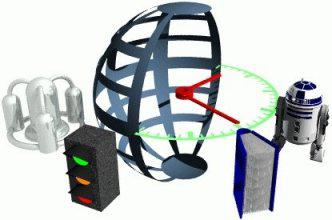
\includegraphics[]{img/test.jpg}
%    \caption{Numele figurii}
%    \label{fig:imag}
%\end{figure}
%
%Fiecare capitol 'incepe pe pagin'a nou'a.
%'In acest capitol se prezint'a tema propriu-zis'a (sub forma unei teme de proiectare sau cercetare, formulat'a exact, cu obiective clare - 2-3 pagini 'si eventuale figuri explicative).
%
%Reprezint'a cca. 10\% din lucrare.

\chapter{Obiectivele Proiectului}
\section{Scop}
Scopul acestui proiect este de a realiza un sistem dedicat de execuție a programelor scrise în limbajul Prolog, urmând a fi folosit de către cercetători și ingineri care activează în domeniul inteligenței artificiale și a programării logice. Acest sistem va fi compus dintr-un procesor special optimizat pentru executarea unui set de instrucțiuni ales din limbajul Prolog, implementat pe un circuit reprogramabil de tipul FPGA, având la bază arhitectura WAM propusă de către David H. D. Warren. El va fi însoțit de o suită de programe compatibile cu sistemele de opererare din familia UNIX, care vor servi ca interfață dintre calculatorul gazdă și noul procesor, FPWAM (FPGA PROLOG WAM).

\section{Obiective generale}
Până la sfârșitul dezvoltării acestui proiect, se urmăresc atingerea următoarelor obiective principale:

\begin{itemize}
\item Studiul în detaliu a mașinii propuse de către David H. D. Warren este imperios necesară deoarece ea va sta la baza procesorului FPWAM.
	\item Identificarea posibilelor instrucțiuni care pot fi optimizate.
	\item După studierea tuturor surselor teoretice, următorul pas va fi acela de a concepe o arhitectură fizică care să exploateze natura paralelă a circuitelor FPGA în implementarea algoritmilor prezenți în mașina WAM.
	\item Arhitectura proiectată să fie scalabilă, astfel încât să permită adăugarea cu ușurință a mai multor procesoare Prolog.
	\item Implementarea efectivă pe un circuit integrat de tip FPGA.
	\item Creșterea frecvenței de ceas prin metode de optimizare a circuitului.
	\item Din cauza faptului că proiectul de față nu iși propune să construiască un compilator de Prolog, este necesară alegerea unuia existent cu care FPWAM să fie compatibil.
	\item Dezvoltarea unui translator din instrucțiuni WAM în cod mașină FPWAM.
	\item Dezvoltarea unei aplicații de comunicare între calculatorul și FPWAM.
	\item Suita de programe dezvoltate să fie compatibile cu sistemele de operare din familia UNIX.
\end{itemize}

\section{Obiective S.M.A.R.T.}
\subsubsection{Principiile S.M.A.R.T.}
De cele mai multe ori scopurile și obiectivele sunt formulate fără o structură anume, având consecințe destul de grave precum imposibilitatea de urmări progresul și lipsa de predictibilitate. Metodologia S.M.A.R.T. de formulare a obiectivelor și a scopurilor este folosită cel mai des în management-ul proiectelor fiind una dintre cele mai eficiente metode în acest sens. Pentru ca un obiectiv să îndeplinească criteriile S.M.A.R.T. el trebuie să îndeplinească următoarele principii:

\begin{itemize}
	\item Specific: Cu cât obiectivul este mai specific, cu atât șansele sunt mai mari să-l obținem. El trebuie să răspundă la întrebări precum ce vreau să obțin exact, unde, cum sau când.
	\item Measurable (măsurabil): Ca un obiectiv să fie măsurabil el trebuie să fie împărțit în elementele măsurabile, rezultatul fiind apreciat după dovezile concrete.
	\item Attainable (realizabil): Este foarte important să punem în balanță efortul, timpul și alte costuri cu profitul și alte priorități pe care le avem.
	\item Relevant: Obiectivul trebuie să contribuie la atingerea scopului dorit.
	\item Time-bound (limitat de timp): Cu toții știm că termenele limită pun oamenii în mișcare, așa că obiectivele trebuie să fie constrânse de timp.
\end{itemize}

\subsubsection{Obiectivele S.M.A.R.T. ale proiectului}
Luând în considerare principiile enumerate mai sus, s-au formulat următoarele obiective S.M.A.R.T. ale proiectului:

\begin{itemize}
	\item Realizarea unui studiu teoretic auspra implementărilor limbajului Prolog:
		\begin{itemize}
			\item S: Studierea și înțelegerea articolului scris de către David H. D. Warren în care introduce pentru prima oară arhitectura WAM. Studierea a altor alternative.
			\item M: Documentarea din cel puțin două surse diferite și schițarea unei sinteze a acestora.
			\item A: Prolog fiind un limbaj de programare popular, se găsesc multe surse din care se pot extrage informații relevante.
			\item R: Studiind soluțiile existente și elaborând o sinteză, putem să punem în balanță avantajele și dezavantajele lor, ducând în final la alegerea optimă.
			\item T: Studiul nu trebuie să depășească 3 luni de zile.
		\end{itemize}
	\item Implementarea procesorului M0 pe FPGA:
	\begin{itemize}
		\item S: În versiunea M0 se urmărește ca procesorul să poată unifica un fapt cu o întrebare Prolog predefinite în memoria de program.
		\item M: Pentru ca acest obiectiv să fie îndeplinit următoarele elemente trebuie să fie implementate: arhitectura de bază formată din memorie și regiștrii,  algoritmul de unificare a faptului cu întrebarea, un set minim de instrucțiuni WAM care să permită unificarea
		\item A: Fiind la îneceputul proiectului, există timp pentru experimente până la definitizarea arhitecturii.
		\item R: Atingerea acestui obiectiv este un pas foarte important deoarece demonstrează viabilitatea unei implementări hardware a limbajului.
		\item T: Cu tot cu implementare și experimente, acest proces nu trebuie să dureze mai mult de 1 lună.
	\end{itemize}
	\item Dezvoltarea suitei de programe pentru mediul de executare a FPWAM:
	\begin{itemize}
		\item S: Suita de programe trebuie să permită compilarea și executarea de programe Prolog pe FPWAM. Modulul de compilare va utiliza GPLC (Gnu Prolog Compiler).
		\item M: Obținerea unor executabilie testate și compatibile cu sistemele de operare din familia UNIX.
		\item A: Compilarea Prolog->WAM este efectuată de către GPLC reducând considerabil complexitatea acestui obiectiv.
		\item R: Datorită acestor programe, interacțiunea dintre FPWAM și utilizator va fi posibilă într-un mod natural și eficient.
		\item T: Funcționalitățile de baza trebuie să fie implementate în maxim 3 zile.
	\end{itemize}
	\item Implementarea procesorului M3 pe FPGA:
	\begin{itemize}
		\item S: În versiunea M3 procesorul va putea să execute orice program Prolog care respectă subsetul selectat de instrucțiuni.
		\item A: Pentru ca acest obiectiv să fie îndeplinit următoarele funcționalități trebuie să fie implementate: mecanismul de apel a unui predicat,  mecanismul de backtracking, 90\% din instrucțiunile WAM.
		\item R: Acest obiectiv duce proiectul aproape de îndeplinirea scopului final. În acest stadiu se pot face comparații și teste amănunțite.
		\item T: Acest obiectiv trebuie să fie îndeplinit la cel puțin 15 zile înaintea de predarea proiectului.
	\end{itemize}
\end{itemize}
	
	
%Documentarea bibliografic'a are ca obiectiv prezentarea stadiului actual al domeniului sau sub-domeniului 'in care se situeaz'a tema. 
%'In redactarea acestui capitol ('in general a 'intregului document) se va 'tine cont de cuno'stin'tele acumulate la disciplinele dedicate din semestrul 2, anul 4 
%(Metodologia 'Intocmirii Proiectelor, etc.), precum 'si la celelalte discipline relevante temei abordate.
%
%Acest capitol reprezint'a cca. 15\% din lucrare.
%
%Referin'tele se scriu 'in sec'tiunea Bibliografie. 
%Formatul referin'telor trebuie s'a fie de tipul IEEE sau asem'an'ator. 
%Introducerea 'si formatarea referin'telor 'in bibliografie, respectiv citarea 'in text, se pot face manual sau folosind instrumentele de lucru men'tionate 'in ultimele paragrafe din acest capitol.
	


%http://allaboutfpga.com/fpga-architecture/

%%In chapter~\ref{ch:analysis} of~\cite{strunk}, which discusses the value of the honeypots, Spitzner presents the advantages and disadvantages of such systems. 
%%
%%
%%'In sec'tiunea {\it Bibliografie} sunt exemple de referin'te pentru articol la conferin'te sau seminarii~\cite{BellucciLZ04}, articol 'in jurnal~\cite{AntoniouSBDB07}, 
%%sau c'ar'ti~\cite{russell1995artificial}. 
%%
%%
%%Referin'tele spre aplica'tii sau resurse online (pagini de internet) trebuie sa includ'a cel pu'tin o denumire sugestiv'a pe l\ia ng'a link-ul propriu-zis~\cite{webpage}, 
%%plus alte informa'tii dac'a sunt disponibile (autori, an, etc.). 
%%Referin'tele care prezint'a doar link spre resursa online se vor plasa 'in subsolul paginii unde sunt referite.
%%Citarea referin'telor 'in text este obligatorie, vezi exemplul de mai jos ('in func'tie de tema proiectului se poate varia modul de prezentare a metodei/aplica'tiei).
%%
%%%'In articolul~\cite{AntoniouSBDB07} autorii prezint'a un sistem pentru ...
%%'In~\cite{AntoniouSBDB07} autorii prezint'a un sistem pentru detec'tia obstacolelor 'in mi'scare folosind stereoviziune 'si estimarea mi'sc'arii proprii. 
%%Metoda se bazeaz'a pe ...{\it trecere 'in revist'a a algoritmilor, structurilor de date, func'tionalitate, aspecte specifice temei proiectului etc}. Discu'tie {\it avantaje - dezavantaje}.
%
%
%'In capitolul~\ref{ch:analysis} al~\cite{russell1995artificial} se prezint'a ...  
%
%
%\section{Titlu}
%\section{Alt titlu}


\chapter{Studiu Bibliografic}

\section{Sisteme de calcul reconfigurabile și FPGA}
În ultimul deceniu, sistemele de calcul reconfigurabile au devenit foarte populare datorită capacității lor de a îmbina flexibilitatea unui produs software cu performanța ridicată a puterii de procesare a componentelor hardware. Acest concept a fost introdus pentru prima oară de către Gerlad Estrin într-un articol publicat în anii 1960-ref. El propunea un sistem format dintr-un procesor standard și o matrice de primitive hardware care putea fi configurată în funcție de necesitatea aplicației. Din cauza limitărilor tehnologice de la acea vreme, acest domeniu nu prea a fost în atenția cercetătorilor. După mai bine de două decenii producătorul de circuite integrate Xilinx inventează și lansează pentru prima oară circuitele field-programmable gate aray (FPGA). Datorită comercializarea acestor circuite și performanțele ridicate ale acestora, domeniul sistemelor reconfigurabile a trecut printr-o perioadă de renaștere în care s-au publicat numeroase articole demonstrând viabilitatea acestor sisteme-ref. 
\subsection{Circuitele integrate FPGA}
Un FPGA este un circuit integrat destinat configurării de către utilizator sau unui arhitect dupa procesul de fabricație. Configurația lor este specificată similar cu cea a circuitelor ASIC (applicațion-specific integrated circuit) utilizând un limbaj de descriere hardware (HDL).\\
Cea mai comună arhitectură pe care o adoptă aceste circuite conține o matrice de blocuri logice configurabile (CLB), celule de intrare/ieșire și canale de rutare. O imagine explicativă se găsește în figura \ref{fig:arhitectura}.
\begin{figure}[ht]
    \centering
    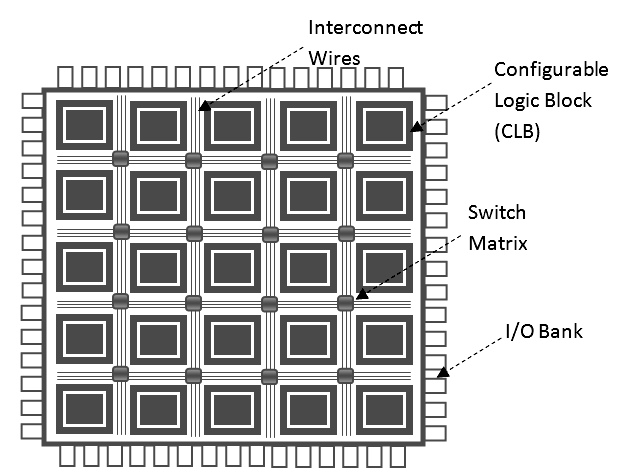
\includegraphics[scale=0.25]{img/FPGA-Architecture.png}
    \caption{Arhitectura unui FPGA (http://allaboutfpga.com/fpga-architecture/
)}
    \label{fig:arhitectura}
\end{figure} 

\subsubsection{Elementele CLB}
Elementele CLB sunt sunt blocurile fundamentale din care sunt formate FPGA-urile. Ele sunt alcătuite din mai multe celule logice (slice-uri). O versiune simplificată a unui slice se găsește în figura \ref{fig:slice}. De regulă el conține:
\begin{itemize}
\item LUT(look-up table) cu 4 intrări
\item Sumator complet
\item Bistabil de tip D
\item Multiplexoare pentru slecția modului \textit{normal sau aritmetic} în combinație cu modul de ieșire \textit{sincron sau asincron}
\end{itemize}

\begin{figure}[ht]
    \centering
    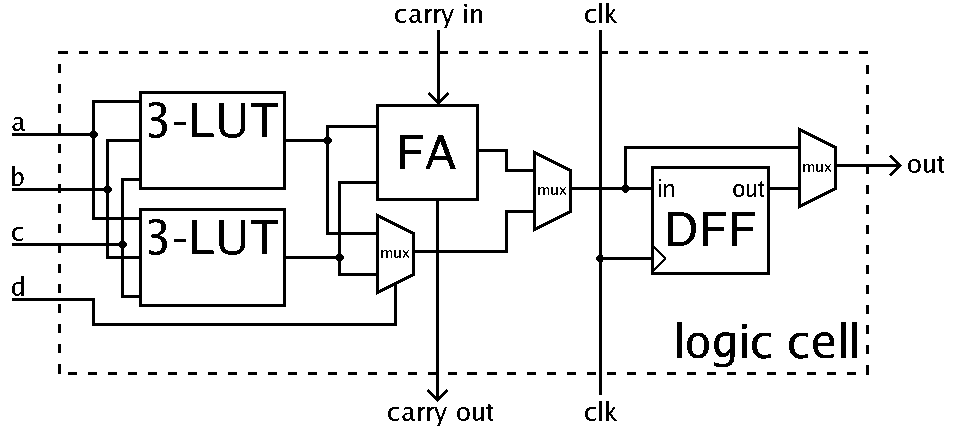
\includegraphics[scale=0.25]{img/FPGA_cell_example.png}
    \caption{SLICE}
    \label{fig:slice}
\end{figure} 

\subsubsection{Elemente de rutare}
Elementele de rutare din FPGA sunt folosite pentru interconectarea blocurilor logice printr-o matrice de fire și comutatoare programabile. O schemă sumară se găsește în figura \ref{fig:rutare}. În general rutarea între elementele programabile este nesegmentată, ceea ce înseamnă că fiecare segment rutat își găsește un capăt într-un bloc logic iar celălalt într-un comutator programabil. Pentru viteze ridicate, unele arhitecturi FPGA folosesc linii de rutare care trec prin mai multe elemente CLB.

\begin{figure}[ht]
    \centering
    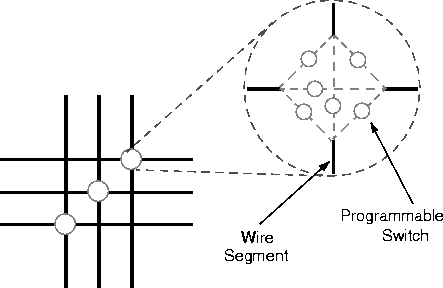
\includegraphics[scale=0.5]{img/switch-box.jpg}
    \caption{Matrice de rutare și comutator programabil}
    \label{fig:rutare}
\end{figure} 

\section{Prolog}
După cum am amintit și în \ref{chap:intro} limbajul Prolog a fost inventat la începutul anilor 1970 de către Alain Colmerauer și colegii lui de la Universitatea din Marseille-ref. El este printre primele limbaje de uz general care au ca paradigmă de baza programarea logică.  Domeniile lui de aplicabilitate sunt de obicei cele din sfera inteligenței artificiale, mai exact a sistemelor bazate pe cunoștințe, sisteme expert, etc-ref.  \\
\subsection{Limbajul Prolog}
Într-un program Prolog pot fi indentificate următoarele construcții de bază:

\begin{enumerate}
	\item fapte
	\item întrebări
	\item termeni
	\item reguli
\end{enumerate}

\subsubsection{Fapte}
În limbajul Prolog putem face afirmații utilizând faptele. Faptele sunt niște itemi ori o relație între itemi. De exemplu:
\begin{verbatim}
	respira(om). %omul respiră
	program_initializat.
\end{verbatim}	
\subsubsection{Întrebări}
Îndată ce faptele au fost definite, Prolog ne permite să interogăm baza de fapte:
\begin{verbatim}
	?-program_initializat.
	yes.
	?-respira(om).
	yes.
	?-respira(carte).
	false.
	?-respira(X), % interogare cu termen de tip variabilă
	X = om
\end{verbatim}
\subsubsection{Termeni}
Termenii în Prolog se grupează în următoarele categorii:
\begin{itemize}
\item simpli
	 \begin{itemize}
	  \item variabile
	  \item constante
	  	\begin{itemize}
		\item atomi
		\item numere
		\end{itemize}
	 \end{itemize}
\item structurați
\end{itemize}
\subsubsection{Reguli}
Prologul permite formularea de reguli de tipul: "Un fapt \textit{a} este adevărat, dacă faptele \textit{b..z} sunt adevărate." Regula Prolog este formată dintr-un \textit{cap} și un \textit{corp} despărțite de simbolul \textit{:-}. Exemplu:
\begin{verbatim}
	a(X):-b(X), c(X), ... ,z(X) %a este adevărat daca b, c ... sunt adevărate 
\end{verbatim}
\subsubsection{Mecanisme}
Spre deosebire de alte limbaje, Prolog are integrate două mecanise ce-l face unic printre alte limbaje de programare.	
\begin{itemize}
\item \textit{Mecanismul de unificare a termenilor.} Doi termeni se unifică doar dacă ei sunt egali sau dacă conțin variable care se pot instanția uniform cu termeni astfel încat cei doi termeni inițiali să fie egai.
\item \textit{Mecanismul de backtracking.} În cazul în care programul ajunge într-o stare în care capul sau corpul unei reguli nu poate fi unificat, mecanismul de backtracking intră în acțiune și reface starea procesului la ultimul punct de alegere și îl execută. Acest procedeu continuă până când unificarea are succes sau nu mai există puncte de alegere, moment în care întrebarea eșuează.
\end{itemize}
\subsection{Arhitectura WAM}
După mai bine de un deceniu de la inventarea limbajului Prolog, în articolul -ref publicat de către David H. D. Warren se descrie o mașină abstractă care este definită printr-un set de instrucțiuni și o arhitectură a memoriei, cunosctă astăzi ca WAM. De atunci, WAM a defenit un standard pentru implementarea limbajului Prolog. Din cauza faptului că Warrren descrie WAM-ul foarte sumar, este dificil pentru un cititor nexperimentat cu limbajul Prolog să înțeleagă arhitectura din lucrarea originală-ref. În -ref Hassan A ̈IT-KACI adresează această problemă publicând o carte sub forma unui tutorial care construiește gradual arhitectura, având în minte principiile după care Warren s-a ghidat.
Arhitectura WAM este una bazată pe stivă, împărtășind similarități cu limbajele imperative: instrucțiuni de tipul call/return, mediu local. Setul de instrucțiuni permite emularea sau translatarea într-un cod mașină nativ.
 %https://www.doc.ic.ac.uk/~shm/Papers/accelfidj.pdf se
 %E. Tick, An overlapped Prolog processor. Artificial Intelligence Center, SRI International, Menlo Park, California 94025, 1983
\section{Abordări similare}
În -ref se propune un sistem hardware implementat pe un circuit integrat de tip FPGA pentru programare logică inductivă. Acest sistem are la bază arhitectura WAM optimizată prin metode de grupare a instrucțiunilor și asignare speculativă. Spre deosebire de abordarea propusă în această lucrare, acest sistem folosește mai multe procesoare WAM interconectate care să lucreze împreună la executarea întrebării Progol. În tabelul 1 din capitolul 5 se demonstrează viabilitatea chiar și unui sistem secvențial, având performanța comparativa cu a unui procesor Pentium III tactat la 450MHz. Dezavantajele acestei abordări sunt tactarea procesorului de Progol la 35MHz-ref, folosirea memoriei RAM distribuite în locul memoriei BlockRAM, forțând ca multe segmente să nu fie ținute în memoria interna a FPGA-ului din cauza lipsei de spațiu. Accesul la segmentele care sunt ținute înafara circuitului vor scădea performanța considerabil.

O altă abordare de implementare hardware a arhitecturii WAM propusă în -ref de către Evan Tick în 1983 încearcă să determine perfomanța maximă pe care o poate atinge o mașină Prolog secvențială. Această abordare nu prea este relevantă, deorece tehnologia a avansat mult de atunci, dar studiul arată că se pot s-au obținut îmbunătățiri de până la 18\% folosind componente hardware standard.




%\label{ch:analysis}
%
%'Impreun'a cu capitolul urm'ator trebuie s'a reprezinte aproximativ 60\% din total.
%
%Scopul acestui capitol este de a explica principiile func'tionale ale aplica'tiei implementate. 
%Aici se va descrie solu'tia propus'a dintr-un punct de vedere teoretic - explica'ti 'si demonstra'ti propriet'a'tile 'si valoarea teoretic'a:
%\begin{itemize}
% \item algoritm utilizat sau propus
%\item protocoale utilizate
%\item modele abstracte
%\item explica'tii/argument'ari logice ale solu'tiei alese
%\item structura logic'a 'si func'tional'a a aplica'tiei.
%\end{itemize}
%
%{\color{red}
%NU SE FAC referiri la implementarea propriu-zis'a. 
%
%NU SE PUN descrieri de tehnologii preluate cu copy-paste din alte surse sau lucruri care nu 'tin strict de proiectul propriu-zis (materiale de umplutur'a).
%}
%
%
%\section{Titlu}
%\section{Alt titlu}
%
\chapter{Analiz'a 'si Fundamentare Teoretic'a}
În acest capitol se va prezenta pe cât posibil bazele teoretice a procesorului care urmează să fie implementat. Arhitectura abstractă WAM este una complicată, având un set de instrucțiuni stufos care nu este intuitiv pentru cititorul nexperimentat cu limbajul Prolog. Pentru înțelegerea în detaliu se recomandă lecturarea cărții -ref. 

În paralel se vor discuta și modificările survenite pentru adaptarea ei la arhitectura care urmeză să fie implementată pe FPGA. O altă parte ce va fi tratată aici este protocolul pentru comunicarea cu calculatorul gazdă, principiile din spatele translatorului WAM-FPWAM și ideea aplicației ce oferă utilizatorului un mediu de exectuare.

Partea legată de arhitectura WAM nu este
\section{Hardware - Arhitectura WAM și soluția propusă}
\subsection{Arhitectura memoriei}
După cum am mai amintit în capitolele anterioare WAM este un procesor bazat pe stivă. În specificația originală, memoria este împărțită în următoarele zone (în ordine crescătoare a spațiului de adrese) :
\begin{enumerate}
	\item \textit{CODE} - zonă de memorie destinată exclusiv păstrarea codului pentru faptele și regulile Prolog.
	\item \textit{HEAP} - zonă de memorie destinată exclusiv păstrarea oricărui tip de termen Prolog.
	\item \textit{STACK} - zonă de memorie despărțită logic în două secțiuni: stivă-AND și stivă-OR. Pe stiva-AND se reține de obicei cadrul local care conține variabilele locale, următorul mediu local și numărul instrucțiunii de întoarecere. Pe stiva-OR se țin informații pentru mecanismul de backtracking. Ele sunt legate de punctul de alegere și informații pentru refacerea stării procesorului la executarea operației backtracking.
	\item \textit{TRAIL} - zonă de memorie destinată ținerii evidenței variabilelor unificate.
	\item \textit{PDL} - zonă de memorie locala destinată algoritmului de unificare a termenilor.
\end{enumerate}
Din motive pe care se vor discuta în capitolele următoare s-a introdus o nouă zonă de memorie care nu este prezentă în lucrarea originală numită \textit{CINDEX}.
\subsection{Regiștrii}
Regiștrii mașinii WAM se împart în două categorii:
\begin{itemize}
	\item de uz general
	\item specializați
\end{itemize}

\subsubsection{Regiștrii de uz general}
Regiștrii de uz general au lățimea cât a unui cuvânt a memoriei și sunt împărțiți logic în următoarele categorii:
\begin{itemize}
	\item regiștrii de variablă - folosiți pentru manipularea termenilor când se construiesc sau se unifică. Ei se notează cu X(i) unde \textit{X} - indică registru de variablă și \textit{i} - indică numărul registrului.
	\item regiștrii de argument - alocați sistematic pentru pregătirea argumentelor a următorului apel de regulă sau predicat. Ei se notează cu A(i) unde \textit{A} - indică registru de argument și \textit{i} - indică numărul registrului.
\end{itemize}
\textit{NOTA BENE} - A și X sunt doar niște notații pentru a indica contextul în care un registru este folosit. A(1) = X(1)

\subsubsection{Regiștrii specializați}
WAM folosește o serie de regiștrii specializați care indică starea procesorului la un moment dat de timp. În continuare se vor prezenta numele lor și o descriere sumară a rolului pe care îl îndeplinesc.
\begin{itemize}
	\item \textit{Registrul P} - folosit să indice adresa instrucțiunii curente.
	\item \textit{Registrul CP} - folosit să indice adresa instrucțiunii care urmează să fie executată la întoarcerea cu success din apelul unei proceduri.
	\item \textit{Registrul S} - folosit ca registru de unificare, reține adresa din zona de memorie HEAP a unui termen.
	\item \textit{Registrul Mode} - folosit pentru a indica modul de execuție, read sau wrtie.
	\item \textit{H} - folosit pentru a reține adresa vârfului zonei de memorie HEAP.
	\item \textit{HB} - folosit pentru a reține reține adresa vârfului zonei de memorie HEAP la timpul ultimului punct de alegere.
	\item \textit{B0} - registru de tăietură.
	\item \textit{B} - folosit pentru a reține adresa începutului punctului de alegere anterior.
	\item \textit{E} - folosit pentru a reține adresa mediului local.
	\item \textit{TR} - folosit pentru a indica vârful zonei de memorie TRAIL.
\end{itemize}

Din cauza că FPWAM suportă doar un subset al limbajului Prolog, registrul B0 care este folosit pentru tăieturi nu este prezent în implementare.

\subsection{Reprezentarea termenilor}
În continuare se va prezenta modalitatea de reprezentare a termenilor Prolog în WAM, repsectiv FPWAM. Pentru stocarea lor vom folosi un bloc global din zona de memorie numită HEAP. FPWAM va suporta patru tipuri de termeni, structuri, variable, constante și liste. Fiecare din acești termeni va avea un marcaj unic pentru a putea fi discriminați pe HEAP. 
\subsubsection{Reprezentarea structurilor}
Structurile sunt niște termeni non-variabili. Pentru a reprezenta o structură de tipul \(f(t_{1}, ... , t_{n})\), vor fi folosite \(n+2\) cuvinte de memorie. Primul va fi un poantor către adresa celui de-al doilea care indică termenul \(f/n\). Evident aceste două cuvinte nu necesită să fie la adrese consecutive. Celelalte \(n\) cuvinte vor fi folosite pentru a reține referințe către rădăcinile subtermenilor \(t_{1} ... t_{n}\). Mai specific, primul cuvânt va fi de forma \(<STR, a>\) ,unde \(STR\) reprezintă marcajul și \(a\) reprezintă adresa la care se află reprezentarea lui \(f/n\). Începând de la adresa \(a\) se va afla întodeauna un bloc contiguu de n+1 cuvinte ce reprezintă numele/aritatea structurii și cele n referințe către subtermenii \(t_{1} ... t_{n}\).
\subsubsection{Reprezentarea variabilelor}
O variabilă va fi indentificată printr-un poantor și va fi reprezentat folosind doar un cuvânt din memorie, adică o celulă variabilă. O asemenea celulă va fi indentificată prin \(<REF, a>\) unde \(REF\) denotă marcajul unei referințe și \(a\) adresa către locația de memorie spre care se face referire. Prin convenție, o variabilă este nelegată dacă ea pointează către ea însuși.
\subsubsection{Reprezentarea constantelor}
O constantă va fi reprezentată folosind doar un cuvând din memorie. O asemenea celulă va fi identificată prin \(<CON, c>\), unde \(CON\) reprezintă marcajul, iar \(c\) reprezintă valoarea constantei.
\subsubsection{Reprezentarea listelor}
Cele mai întâlnite structuri de date în programele Prolog sunt listele, fapt pentru care se vor introduce marcaje speciale pentru acestea. O element dintr-o listă este indentificat prin perechea de celule \(<LIS, a>\), unde  \(LIS\) reprezintă marcajul prin care se discriminează lista, iar celula de la adresa \(a\) unde se găsește referința către data elementului din listă. Pentru a respecta contiguitatea termenilor, aceste prerechi trebuie să fie la adrese consecutive în memorie până la terminarea listei care este indicată prin constanta \(<CON, NIL>\).
\subsubsection{Exemple de reprezentări ai termenilor}
În \ref{repr:termen1} se arată reprezentarea termenului \(f(Z, h(Z, W),f(W))\) pe HEAP.  În acest exemplu se demonstrează reprezentarea variabilelor nelegate și a structurilor. De observat aici este contiguitatea subtermenilor a structurilor, cât și nerespectarea formatului de \(n+2\) celule. Această mică optimizare se întâmplă doar când faptul urmează să fie apelat dintr-o  regulă, celulele de tip \(<STR, a>\) aflându-se în regiștrii de argument. Această optimizare va fi discutată în capitolele următoare. În toate celelalte cazuri, celulele anterior amintite vor exista pe HEAP. 

În \ref{repr:termen2} se demonstrează reprezentarea unei liste \([\_, \_, f(b), a]\), în care toate primele două elemente sunt niște variabile nelegate iar celelalte un termen structurat și o constantă. De observat în acest exemplu este contiguitatea listei care se termină prin constanta specială \(<CON, NIL>\) și existența celulei \(<STR, \_>\).

\begin{figure}
\begin{center}
\begin{tabular}{c|c|c|}
\cline{2-3}
0 & \multicolumn{2}{|c|}{\(h/2\)} \\
\cline{2-3}
1 & REF & 1 \\
\cline{2-3}
2 & REF & 2 \\
\cline{2-3}
3 & \multicolumn{2}{|c|}{\(f/1\)} \\
\cline{2-3}
4 & REF & 2 \\
\cline{2-3}
5 & \multicolumn{2}{|c|}{\(p/3\)} \\
\cline{2-3}
6 & REF & 1 \\
\cline{2-3}
7 & STR & 0 \\
\cline{2-3}
8 & STR & 3 \\
\cline{2-3}
\end{tabular}
\end{center}
\caption{Reprezentare a termenului \(f(Z, h(Z, W),f(W))\)} \label{repr:termen1}
\end{figure}

\begin{figure}
\begin{center}
\begin{tabular}{c|c|c|}
\cline{2-3}
0 &LIS & 1 \\
\cline{2-3}
1 & REF & 1 \\
\cline{2-3}
2 & LIS & 3 \\
\cline{2-3}
3 & REF & 3 \\
\cline{2-3}
4 & LIS & 5 \\
\cline{2-3}
5 & STR & 10\\
\cline{2-3}
6 & LIS & 7 \\
\cline{2-3}
7 & CON & a \\
\cline{2-3}
8 & CON & NIL \\
\cline{2-3}
9 & STR & 10 \\
\cline{2-3}
10 & \multicolumn{2}{|c|}{\(f/1\)} \\
\cline{2-3}
11 & CON & b \\
\cline{2-3}
\end{tabular}
\end{center}
\caption{Reprezentarea unei liste \([\_, \_, f(b), a]\)} \label{repr:termen2}
\end{figure}

\subsection{Setul abstract de instrucțiuni și operațiile auxiliare}
Cea mai bună modalitate de a înțelege un procesor este de a-i cunoște instrucțiunile și cum ele operează. Din cauza faptului că arhitectura WAM conține un minimum de 30 de instrucțiuni, în acest subcapitol se va încerca atingerea tutoror tipurilor de instrucțiuni cu exemple și explicații relevante din fiecare categorie. Deoarece FPWAM nu surpotă instrucțiuni de tăietură, ele nu vor fi explicate în acest subcapitol. 

Instrucțiunile mașinii WAM se încadrează în 7 categorii:
\begin{enumerate}
	\item instrucțiuni de tipul PUT
	\item instrucțiuni de tipul GET
	\item instrucțiuni de UNIFICARE
	\item instrucțiuni de CONTROL
	\item instrucțiuni de ALEGERE
	\item instrucțiuni de INDEXARE
	\item instrucțiuni de CUT
\end{enumerate}
  



\chapter{Proiectare de Detaliu 'si Implementare}

'Impreun'a cu capitolul precedent reprezint'a aproximativ 60\% din total.

Scopul acestui capitol este de a documenta aplica'tia dezvoltat'a 'in a'sa fel 'inc\ia t dezvoltarea 'si 'intre'tinerea ulterioar'a s'a fie posibile. 
Cititorul trebuie s'a identifice func'tiile principale ale aplica'tiei din ceea ce este scris aici.
Capitolul ar trebui sa con'tin'a (nu se rezum'a neap'arat la):
\begin{itemize}
 \item schema general'a a aplica'tiei
\item descrierea fiec'arei componente implementate, la nivel de modul
\item diagrame de clase, clase importante 'si metode ale claselor importante.
\end{itemize}


\chapter{Testare 'si Validare}

Aproximativ 5\% din total

\section{Titlu}
\section{Alt titlu}

\chapter{Manual de Instalare 'si Utilizare}

'In sec'tiunea de Instalare trebuie s'a detalia'ti resursele software 'si hardware necesare pentru instalarea 'si rularea aplica'tiei, precum 'si o descriere pas cu pas a procesului de instalare. 
Instalarea aplica'tiei trebuie s'a fie posibil'a pe baza a ceea ce se scrie aici.

'In acest capitol trebuie s'a descrie'ti cum se utilizeaz'a aplica'tia din punct de vedere al utilizatorului, f'ar'a a men'tiona aspecte tehnice interne.
Folosi'ti capturi ale ecranului 'si explica'tii pas cu pas ale interac'tiunii. 
Folosind acest manual, o persoan'a ar trebui s'a poat'a utiliza produsul vostru.

\section{Titlu}
\section{Alt titlu}

\chapter{Concluzii}

Cca. 5\% din total.
Capitolul ar trebui sa con'tin'a (nu se rezum'a neap'arat la):
\begin{itemize}
 \item un rezumat al contribu'tiilor voastre
\item analiz'a critic'a a rezultatelor ob'tinute
\item descriere a posibilelor dezvolt'ari 'si 'imbun'at'a'tiri ulterioare
\end{itemize}


\section{Titlu}
\section{Alt titlu}


%\addcontentsline {toc}{chapter}{Bibliography} 
\bibliographystyle{IEEEtran} 
\bibliography{thesis}%same file name as for .bib

\include{apendix}

\end{document}
